\section{Results}

The results of the study were disappointing to say the least. Timing data for each of the kalman filter versions is shown in figure 3; figure 4 is the same graph without the Parallel-Kalman, OMP-LA version to make it more legible. These graphs show that the Kalman update suffers a 10x or 100x slow down compared to the sequential code. It is clear that other methods of performance improvement should be considered for this part of the program.

In figures 5 and 6 the results of the linear algebra only experiments are shown. These again demonstrate that attempts to parallelize the operations using OpenMP were largely unsuccessful, but the Intel compiler's parallel flag did improve the performance of the Linear Algebra operations. 


\begin{figure}[h]
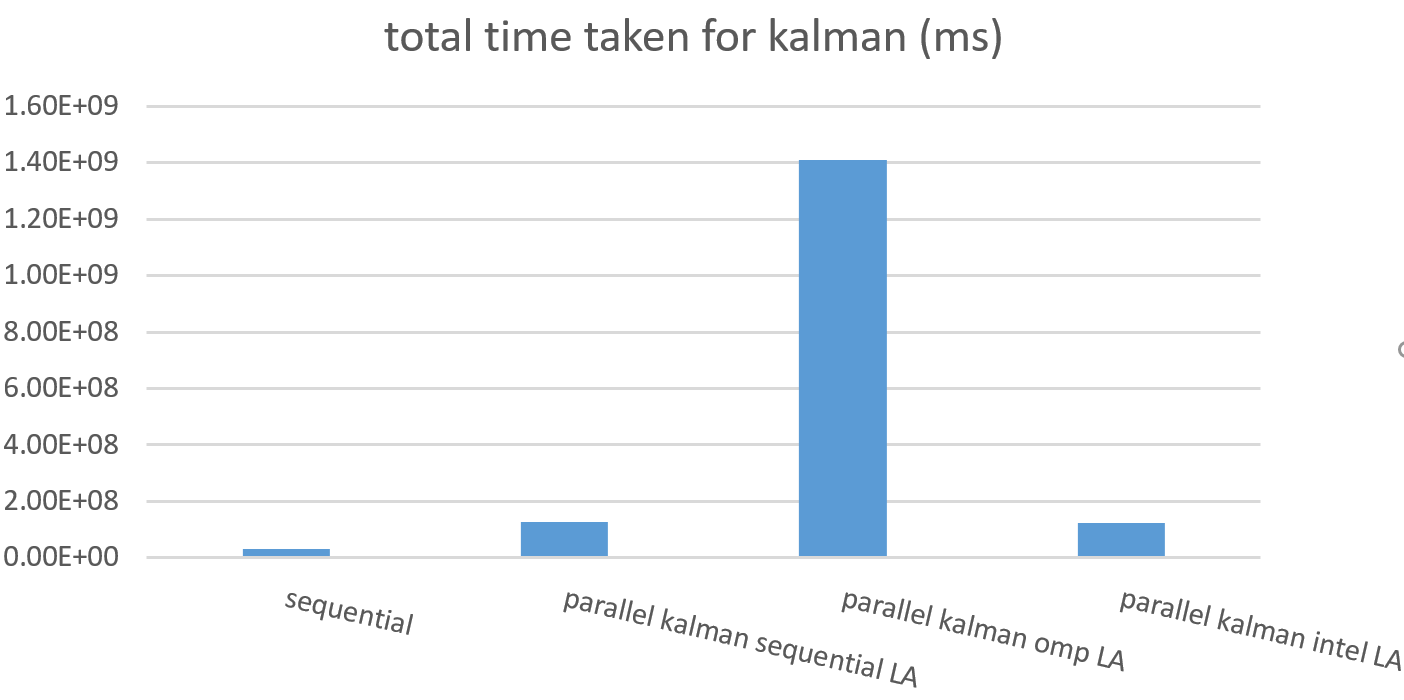
\includegraphics[width=\textwidth]{results1.png}
\label{fig:all_kalman}
 \caption{Timing results of each Kalman implementation}
\end{figure}

\begin{figure}[h]
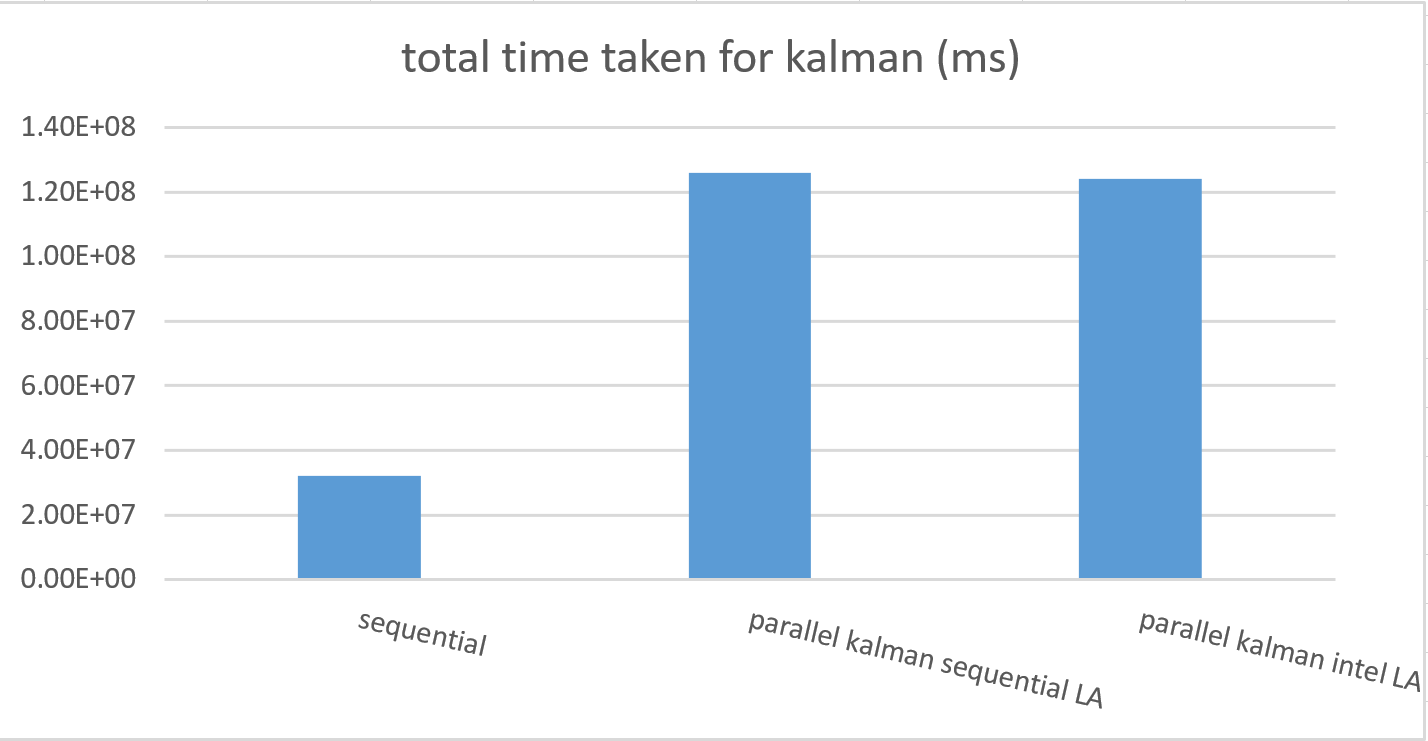
\includegraphics[width=\textwidth]{results2.png}
\label{fig:some_kalman}
 \caption{Timing results of each Kalman implementation}
\end{figure}


\begin{figure}[h]
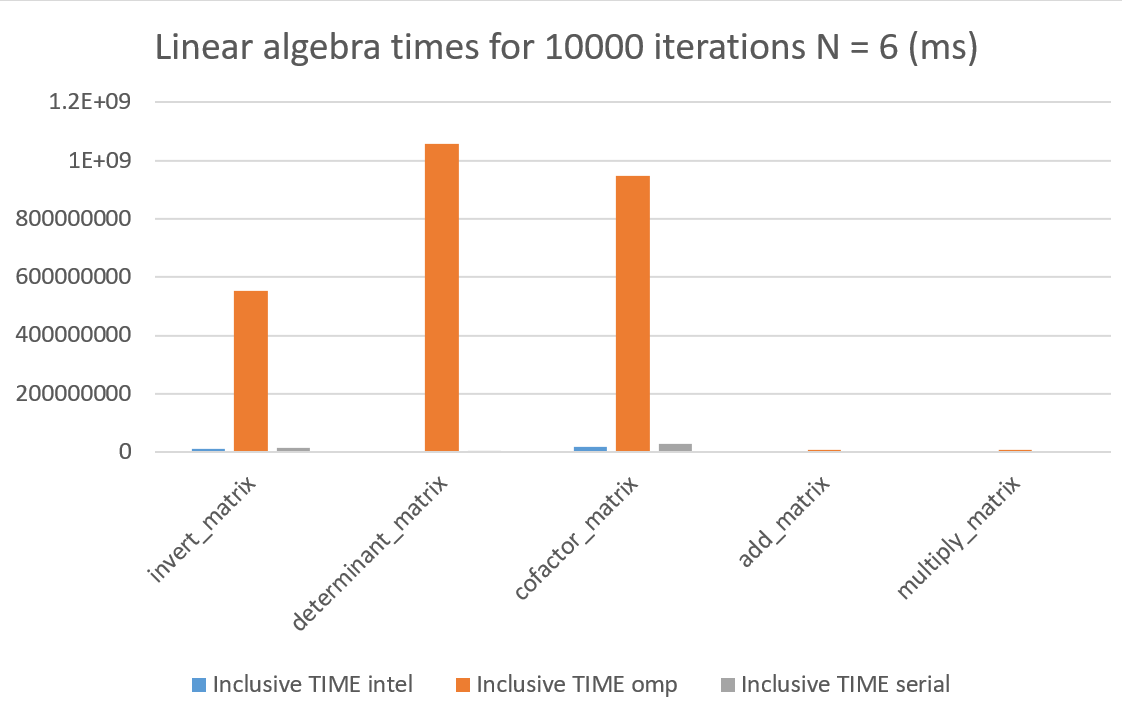
\includegraphics[width=\textwidth]{results_LA1.png}
\label{fig:all_linear}
 \caption{Timing results of each Linear Algebra experiments}
\end{figure}

\begin{figure}[h]
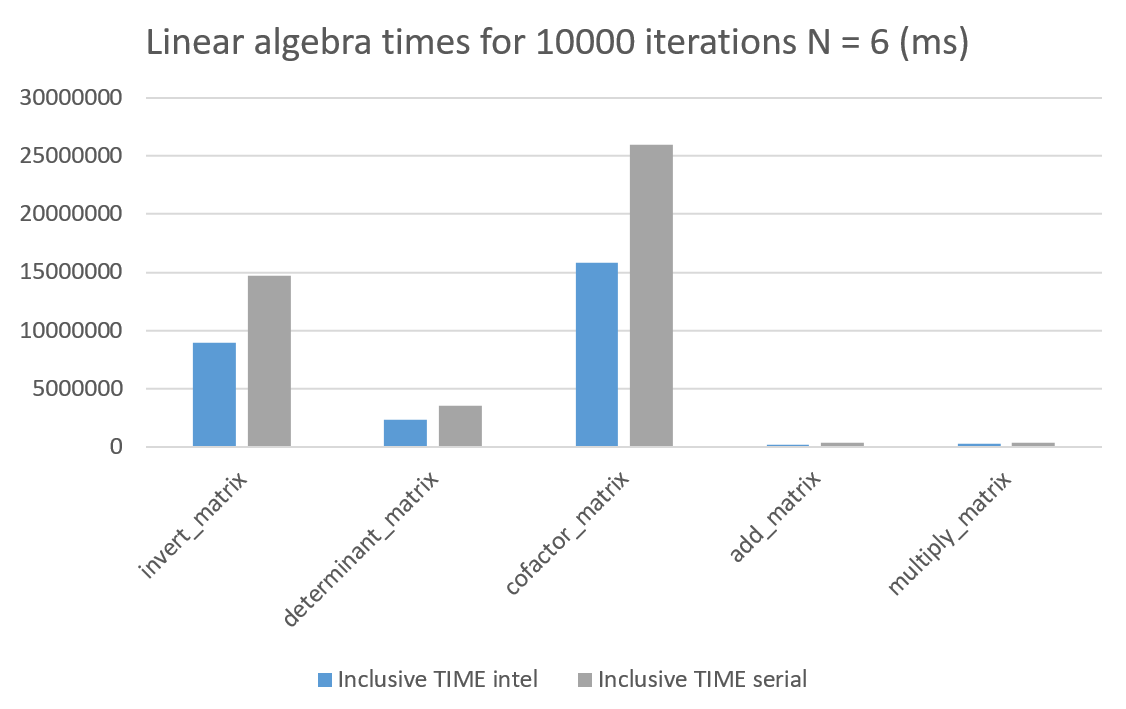
\includegraphics[width=\textwidth]{results_LA2.png}
\label{fig:some_linear}
 \caption{Timing results of each Linear Algebra experiments}
\end{figure}


There are several possible reasons for the slowdown. First, the matrices involved are quite small, so the overhead of creating the threads may overwhelm the gains causing the slowdown. The extreme case of parallelizing Kalman filters and Linear algebra with OpenMP results in nested thread that adds to scheduling overheads as well. 

The other primary suspect for poor performance is programmer error; the DAG was incorrectly designed and the error not noticed until the writing of this report. Figure 2 indicates the dependencies of the system with those in red left out of the implementation. It seems likely that OpenMP recognized the dependence and refused to parallelize that section.

Notably the Intel parallelization did not create new threads but still managed to improve over the serial linear algebra. This is likely the result of vectorization of some of the matrix operations. Although these improvements did not translate to the Kalman filter it suggests that there is more work to be done in that area.

\section{Alternatives and Future Work}
While these experiments produced largely negative results, there are still options available to improve the performance of  the system. The Intel compiler results suggest that vectorization provides good opportunities for improvement. This could be furthered with unrolling loops, removing dependencies, and rearranging data to make it slightly more friendly to vector instructions. 

This project presented a good learning opportunity for those involved. It was a clear case study for the importance of analyzing a problem theoretically before diving into the programming. Had the authors done a better job of this prior to the project we would have not attempted to parallelize the matrix operations through threads, but focused on the potential for pipelining the broader application. 

